% Put labels, etc., on figures using PSTricks.
% Use dvips -E <file>.dvi -o <file>.eps to create encapsulated PostScript.
%
\documentclass[12pt]{article}
\usepackage{graphicx}
\usepackage{pstricks}
\pagestyle{empty}

\begin{document}
\rput(5,-5){
\rput(.1,-.1){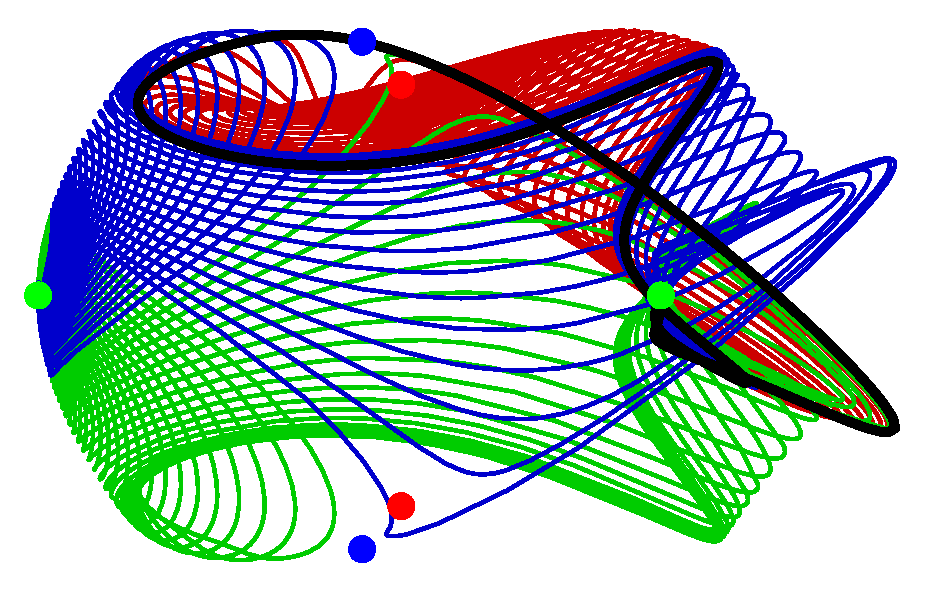
\includegraphics{../../rpo_ks/figs_pst/KS22hetero.eps}}

\huge

\psframe*[linecolor=white](-6.5,6)(-5.5,7)
\psframe*[linecolor=white](6,-6.5)(7.2,-5.5)

\rput(-1.5,4.7){E$_3$} \rput(-7.9,0){E$_2$}

\rput(-1.5,-5.2){$\tau_{1/2}$E$_3$}

\psline[linewidth=2pt]{->}(-0.5,4.7)(-0.95,3.5)\rput(0,5){E$_1$}
\psline[linewidth=2pt]{->}(5.9,2.9)(3.4,-0.1)\rput(6.4,3.4){$\tau_{1/4}$E$_2$}
\psline[linewidth=2pt]{->}(0.4,-4.5)(-0.95,-3.8)\rput(1.7,-4.7){$\tau_{1/2}$E$_1$}


% Use grid command below to place objects at specified coordinates.
%\psgrid[subgriddiv=1,griddots=10](-8,-8)(10,10)
}
\end{document}
